\chapter{基于深度嵌入卷积聚类方法的地海杂波无监督分类}
\section{引言}
由于有监督学习需要对大量的数据进行打标签,这个过程通常需要花费大量的时间与精力。无监督学习也即聚类算法,由于其不需要数据标签,因此国内外学者对各个领域的聚类算法进行了广泛研究,产生了各种不同类型的聚类算法,例如层次聚类\cite{heller2005bayesian},基于质心的聚类方法\cite{lloyd1982least}、基于图的聚类方法\cite{shi2000normalized}、基于回归模型\cite{wang2013multi}的聚类方法以及基于子空间\cite{agrawal1998automatic}的聚类方法。
另一方面,这些聚类方法一般可以分为两类,即生成式和判别式聚类算法。像K均值和高斯混合模型\cite{biernacki2000assessing}这样的生成算法使用特征空间的几何特性来明确地表示簇,并且通过输入数据的统计分布来对分类进行建模。
与生成式聚类算法不同,判别式方法直接使用分离超平面来识别类别,而不管数据的分布是怎样的。信息论\cite{li2004minimum},支持向量机\cite{xu2005maximum}和图谱论\cite{ng2002spectral}算法是判别式聚类模型的例子。
一般认为,判别式模型与其对应的生成式模型相比往往具有更好的结果,因为他们对数据分布的假设较少,直接将聚类分开,但是他们的训练可能会出现过拟合或陷入局部最优解的问题出现\cite{raina2004classification}。
我们的DECC算法也是一种判别式聚类算法,但它受益于自编码器的辅助重构任务,以缓解我们判别式聚类算法的训练中的这个问题。

虽然,聚类问题已经在各种领域进行了应用研究,但是传统的聚类算法的性能收到数据维数以及数据量的影响,会产生维数灾难的问题。
为了解决计算复杂度的问题,以往的研究往往首先将数据投影到一个低维流形中,然后将嵌入的数据聚类到这个新的子空间中\cite{roth2004feature}。处理大规模的数据集,也有一些研究只选择数据点的一个子集来加速聚类过程\cite{shinnou2008spectral}。

就要在特征空间中数据的局部属性而言,基本的思路通过向目标函数添加先验知识来考虑稀疏性或图形约束\cite{tian2014learning}。这类算法可以分为两个阶段:特征学习和聚类。

特征学习指的是一类试图利用一组基本向量或特征来描述一个数据集的学习方法,并且通常这个表示是稀疏的。
在实践中,有很多不同的算法可以进行特征学习,包括自编码器、k-均值聚类、高斯混合模型和受限玻尔兹曼机(RBM)\cite{coates2011analysis}。
这些方法都倾向于学习类似的局部滤波器字典\cite{coates2011analysis},例如用于自然图像的Gabor类边缘滤波器,或者用于MNIST数字数据集的书写笔划。
虽然RBM是可以从数据生成分布中抽样的生成模型\cite{hinton2010practical},但是自编码器被训练来优化它们对输入数据的重构。

自编码器(Autoencoder, AE)是一种简单的神经网络,旨在尽可能减少失真的情况下将输入转换成输出。
虽然在概念上简单,但其在机器学习中起着重要的作用。
自编码器是20世纪80年代由Hinton和PDP小组\cite{rumelhart1985learning}首次提出的,用输入数据作为标签来解决无监督反向传播的问题。
自编码器与Hebbian学习规则\cite{hebb2005organization}一起为无监督学习提供了一个基本的范例,
并开始解决如何以自组织的方式协调局部事件引起的变化去产生全局学习和智能表现。%Autoencoders provide one of the fundamental paradigms for unsupervised learning and for beginning to address the mystery of how synaptic changes induced by local biochemical events can be coordinated in a self-organized manner to produce global learning and intelligent behavior.

最近,自编码器在深度架构方法\cite{hinton2006reducing,hinton2006fast,bengio2007scaling,erhan2010does}中再次占据了中心位置,
,特别是形式上类似受限玻尔兹曼机的自编码器,以堆栈形式组织,然后以无监督的方式自下而上地进行训练,随后是以有监督学习的方式训练顶层并微调整个架构。
考虑到自下而上训练阶段对于最终的任务是不可知的,因此显然可以用于迁移学习方法。并且实际的实验已经证明这些深层次的体系结构可以在一些具有挑战性的分类和回归问题上得到最优的结果。

尽管广大学者已经产生了很大的兴趣,但除了文献\cite{montufar2011refinements,sutskever2008deep,baldi1989neural}等,对自编码器和深层架构的理论认识的文章还很少。除此之外,使用深度一词可能会造成更多混淆。
从计算机科学的角度来看,深层结构应该对于一些小的$\alpha> 0,$有$n\alpha$个多项式大小的层,其中$n$是输入向量的大小\cite{clote2013boolean}。
但是在Hinton等人\cite{hinton2006reducing,hinton2006fast}描述的架构中并不是这种情况,似乎有恒定或最好的对数深度。对于计算机视觉、语音识别和其他典型问题,有限和对数的深度之间的区别很小,几乎可以忽略。
文献\cite{baldi2012autoencoders}对自编码器的理论进行了描述,提出了一个用自编码器解决线性与非线性问题的通用的数学框架。

后来,文献\cite{xie2016unsupervised}提出了共同完成特征学习和聚类的算法。
深度嵌入聚类算法\cite{xie2016unsupervised}以自学习的方式定义了一个有效的目标函数。定义的聚类损失函数用于同时更新网络和聚类中心的变换参数。
但是,他们忽略了数据属性的保持性,这可能导致特征空间的破坏。我们通过保留数据生成分布的局部结构并结合卷积层来改进DEC算法。% However, they ignore the preservation of data properties, which may lead to the corruption of feature space. We improve DEC algorithm by preserving local structure of data generating distribution and by incorporating convolutional layers.
深度聚类算法中使用最广泛的神经网络是堆栈自编码器\cite{xie2016unsupervised}。
SAE需要逐层预训练,然后以端对端(end-to-end)的方式进行微调。
当层次更深时,预训练过程是十分耗时的。此外,SAE是建立在全连接的层次上,对于处理局部信息是无效的。
文献\cite{dundar2015convolutional}的工作是第一个在不需要预训练的情况下直接以端到端的方式直接训练CAE的试验。

\section{卷积自编码网络}
\subsection{自编码器}

自编码器是一种利用隐层用来重构输入的神经网络。其模型如图\ref{fig:ae}所示,它由编码器(Encoder)和解码器(Decoder)两部分组成,本质上是对输入信号的某种变换。编码器将输入信号$x\in[0,1]^{n_x}$编码到某个隐层的表示$h\in[0,1]^n_h$,然后解码器再将$h$解码为输出$x'\in[0,1]^{n_x}$。通过最小化$x$与$x'$之间的差距,可以训练得到一个特征表示的映射$h$,其可以用来重构输入。
\begin{figure}
	\centering
	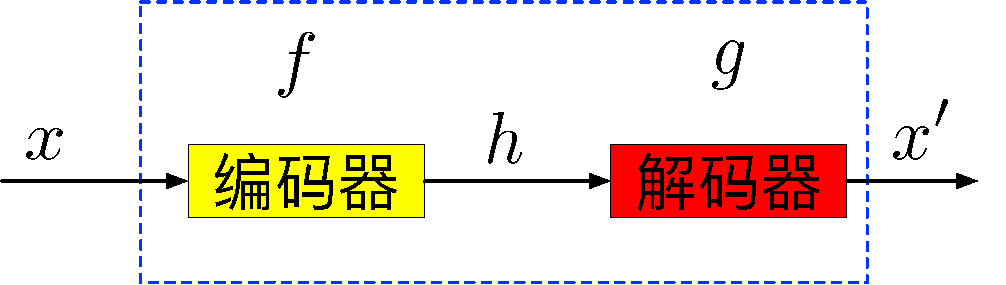
\includegraphics[width=\textwidth]{figures/AE/ae}
	\caption{自编码器模型}
	\label{fig:ae}
\end{figure}
编码和解码公式如下:
\begin{align}
	h_j &= sigm(b_j+\sum_{i=1}^{n_x}w_{ij}x_i) \\
	x_i' &= sigm(a_i+\sum_{j=1}^{n_h}w_{ij}'h_j)
\end{align}
其中,$n_x$和$n_h$分别为输入表示和隐层表示的维数,$sigm(x)=\frac{1}{1+e^{-x}}$是logistic损失函数,$\textbf{W}=[w_{ij}]$和$\textbf{W'}=[w'_{ij}]$为权重矩阵,$\textbf{a}=[a_i]$和$\textbf{b}=[b_j]$为偏差向量。

对于一组具有$N$个输入向量的给定训练数据集,
设每个训练向量为 $x^{(n)}$ 可以被映射到一个隐藏层表示 $h^{(n)}$, 其重构表示为 $x′^{(n)}$. 模型参数$\Theta={\textbf{W},\textbf{a},\textbf{b}}$通过最小化其损失函数进行求取,一般利用均方误差损失函数(mean squared error, mse):
\begin{align}
	J(\theta) &= \frac{1}{N}\sum_{n=1}^N||x^{(n)}-x'^{(n)}||_2^2 \\
	\theta^* &= arg\min\limits_{\theta} J(\theta)  \label{equ:mse}
\end{align}
通常,使用随机梯度下降(SGD)或其余基于梯度的优化算法来对公式\ref{equ:mse}求解。

在此基础上,学者对自编码器进行了各种改进,提出了可以学习输入空间中扰动不变的特征的压缩自编码器\cite{rifai2011contractive}、
提供有效的变分方法进行训练和生成推理的变分自编码器\cite{kingma2013auto}
以及可以基于连续的数据流在运行中添加或合并隐藏单元的在线增量自编码器 \cite{zhou2012online}。

\subsection{卷积自编码器}
传统的自编码网络只有一个隐藏层,只能学习出一种特征变化,
于是Bengio\cite{bengio2007greedy}等人在2007年的
仿照stacked RBM构成的DBN,提出堆栈自编码器(Stacked Auto-Encoder, SAE),为非监督学习在深度网络的应用又添了猛将。
堆栈自编码器的基本模型可以参看图\ref{fig:sae},其通过逐层非监督学习的预训练,也即逐层初始化(Layer-wise Pre-training),来初始化深度网络的参数,替代传统的随机初始化的方法。预训练完毕后,利用训练参数,再进行监督学习训练。

\begin{figure}
	\centering
	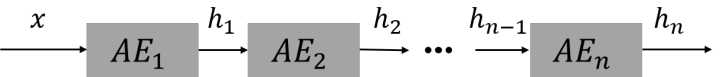
\includegraphics[width=\textwidth]{figures/AE/sae}
	\caption{堆栈自编码器模型}
	\label{fig:sae}
\end{figure}

全连接自编码器和深度自编码器都忽略了数据的局部结构信息。
这在处理实际大小的输入时不仅是一个问题,而且在参数中引入冗余,迫使每个特征是全局的。
然而,在视觉和对象识别领域最成功的模型\cite{lowe1999object}均主要利用了在整个输入空间发生重复的局部特征。
基于此,文献\cite{masci2011stacked}提出了一种卷积自编码器(Convolutional Auto-Encoders, CAE)。
卷积自编码器不同于传统的自编码器,它们的权重在输入向量中的所有位置之间共享,从而可以保持空间局部性。
因此重建结果是隐藏局部特征的线性组合。

CAE架构直观地类似于AE的架构,除了权重是共享的。对于输入x,第k个特征映射的隐藏表示由下式给出
\begin{equation}
	h^k=\sigma(x*W^k+b^k)
	\label{equ:cae1}
\end{equation}
A single bias per latent map is used, as we want each filter to specialize on features of the whole input (one bias per pixel would introduce too many degrees of freedom).
其中偏差也是全局共享的,$\sigma$是激活函数(我们在我们所有的实验中使用缩放的双曲正切),$*$表示二维卷积。
因为我们希望每个滤波器专注于整个输入空间的特征,另一方面如果每个数据点一个偏差将引入太多的自由度,所以对每一个隐藏层使用相同的偏差。
重建过程由下式计算
\begin{equation}
	y=\sigma(\sum_{k \in H}h^k * \tilde{W}^k + c)
	\label{equ:cae2}
\end{equation}
同样的对于每一个输入通道只有一个偏差$c$。 $H$表示潜在特征图的组。
$\tilde{W}$ 标识权重的两个维度上的翻转操作。
公式\ref{equ:cae1}和\ref{equ:cae2}中的2D卷积操作由上下文决定。
一个$m\times m$矩阵和一个$n\times n$矩阵的卷积结果可能是$(m+n− 1) \times (m + n − 1)$(full convolution)也可能是$(m − n + 1) \times  (m − n + 1)$(valid convolution)。
其损失函数为最小均方误差(mean squared error, MSE)
\begin{equation}
	E(\theta) = \frac{1}{2n}\sum_{i=1}^n(x_i-y_i)^2
\end{equation}
就像标准的神经网络一样,反向传播算法被用来计算相对于参数的误差函数的梯度。 这可以通过使用以下公式的卷积运算容易地得到:
\begin{equation}
	\frac{\partial E(\theta)}{\partial W^k}=x * \delta h ^k+\tilde{h}^k * \delta y
\end{equation}
$\delta h$ 和 $\delta y$分别是隐藏层状态和重构结果的变化量。 然后使用随机梯度下降来更新权重。

我们的主要思想是,CAE有利于学习数据的局部结构,避免特征空间的失真。

我们介绍了一种用于分层特征提取的无监督方法,卷积自编码器。
虽然CAE的过完备隐藏表示使得学习比标准自编码器更难,但是我们可以通过添加池化层加强其稀疏性而不需要通过反复试验来设置正则化参数。

\section{深度嵌入卷积聚类方法}
深层嵌入式聚类(Deep Embedding Clustering, DEC)\cite{xie2016unsupervised}算法提供了一种无监督的方式学习特征表示和聚类的思路,通过联合优化神经网络和聚类中心提高了聚类算法的性能和鲁棒性。但是,该算法由于利用了堆栈自编码器,无法利用数据的局部特征信息,
因此本章在此基础上提出了深度嵌入卷积聚类方法(Deep Embedding Convolution Clustering, DECC),利用卷积自编码器代替传统的堆栈自编码器。
\subsection{深度嵌入卷积聚类方法结构}
首先对于问题进行形式化描述,假设需要将$N$个样本$X=[x_1,\dots,x_N]$聚为$K$个类别,其聚类中心点为$\mu_1,\dots,\mu_K$,其中每一个样本$x_i\in \mathbb{R}^{d_x}$,由于对于维数较大的样本会产生维数灾难的问题,因此需要引入一个嵌入函数$\varphi_W: X \rightarrow Z$,可以将原始样本映射到嵌入子空间$Z=[z_1,\dots,z_N]$,其中$z_i\in \mathbb{R}^{d_z}$的维数远小于原始样本的维数,也即$d_z<<d_x$。

本章利用卷积自编码器作为嵌入函数对原始样本进行降维,其基本结构如图 xxx 所示。
通过三次卷积操作充分提取输入样本的特征,我们在所有层上均利用ReLU激活函数,并且在编码器后以相反的顺序放置解码器,由于编码器为卷积操作,故解码器为逆卷积(Deconvolution)。在编码器与解码器中间添加嵌入层,该层的结果被用于进行聚类操作。DECC的结构如图 \ref{fig:decc} 所示。

\begin{figure}
	\centering
	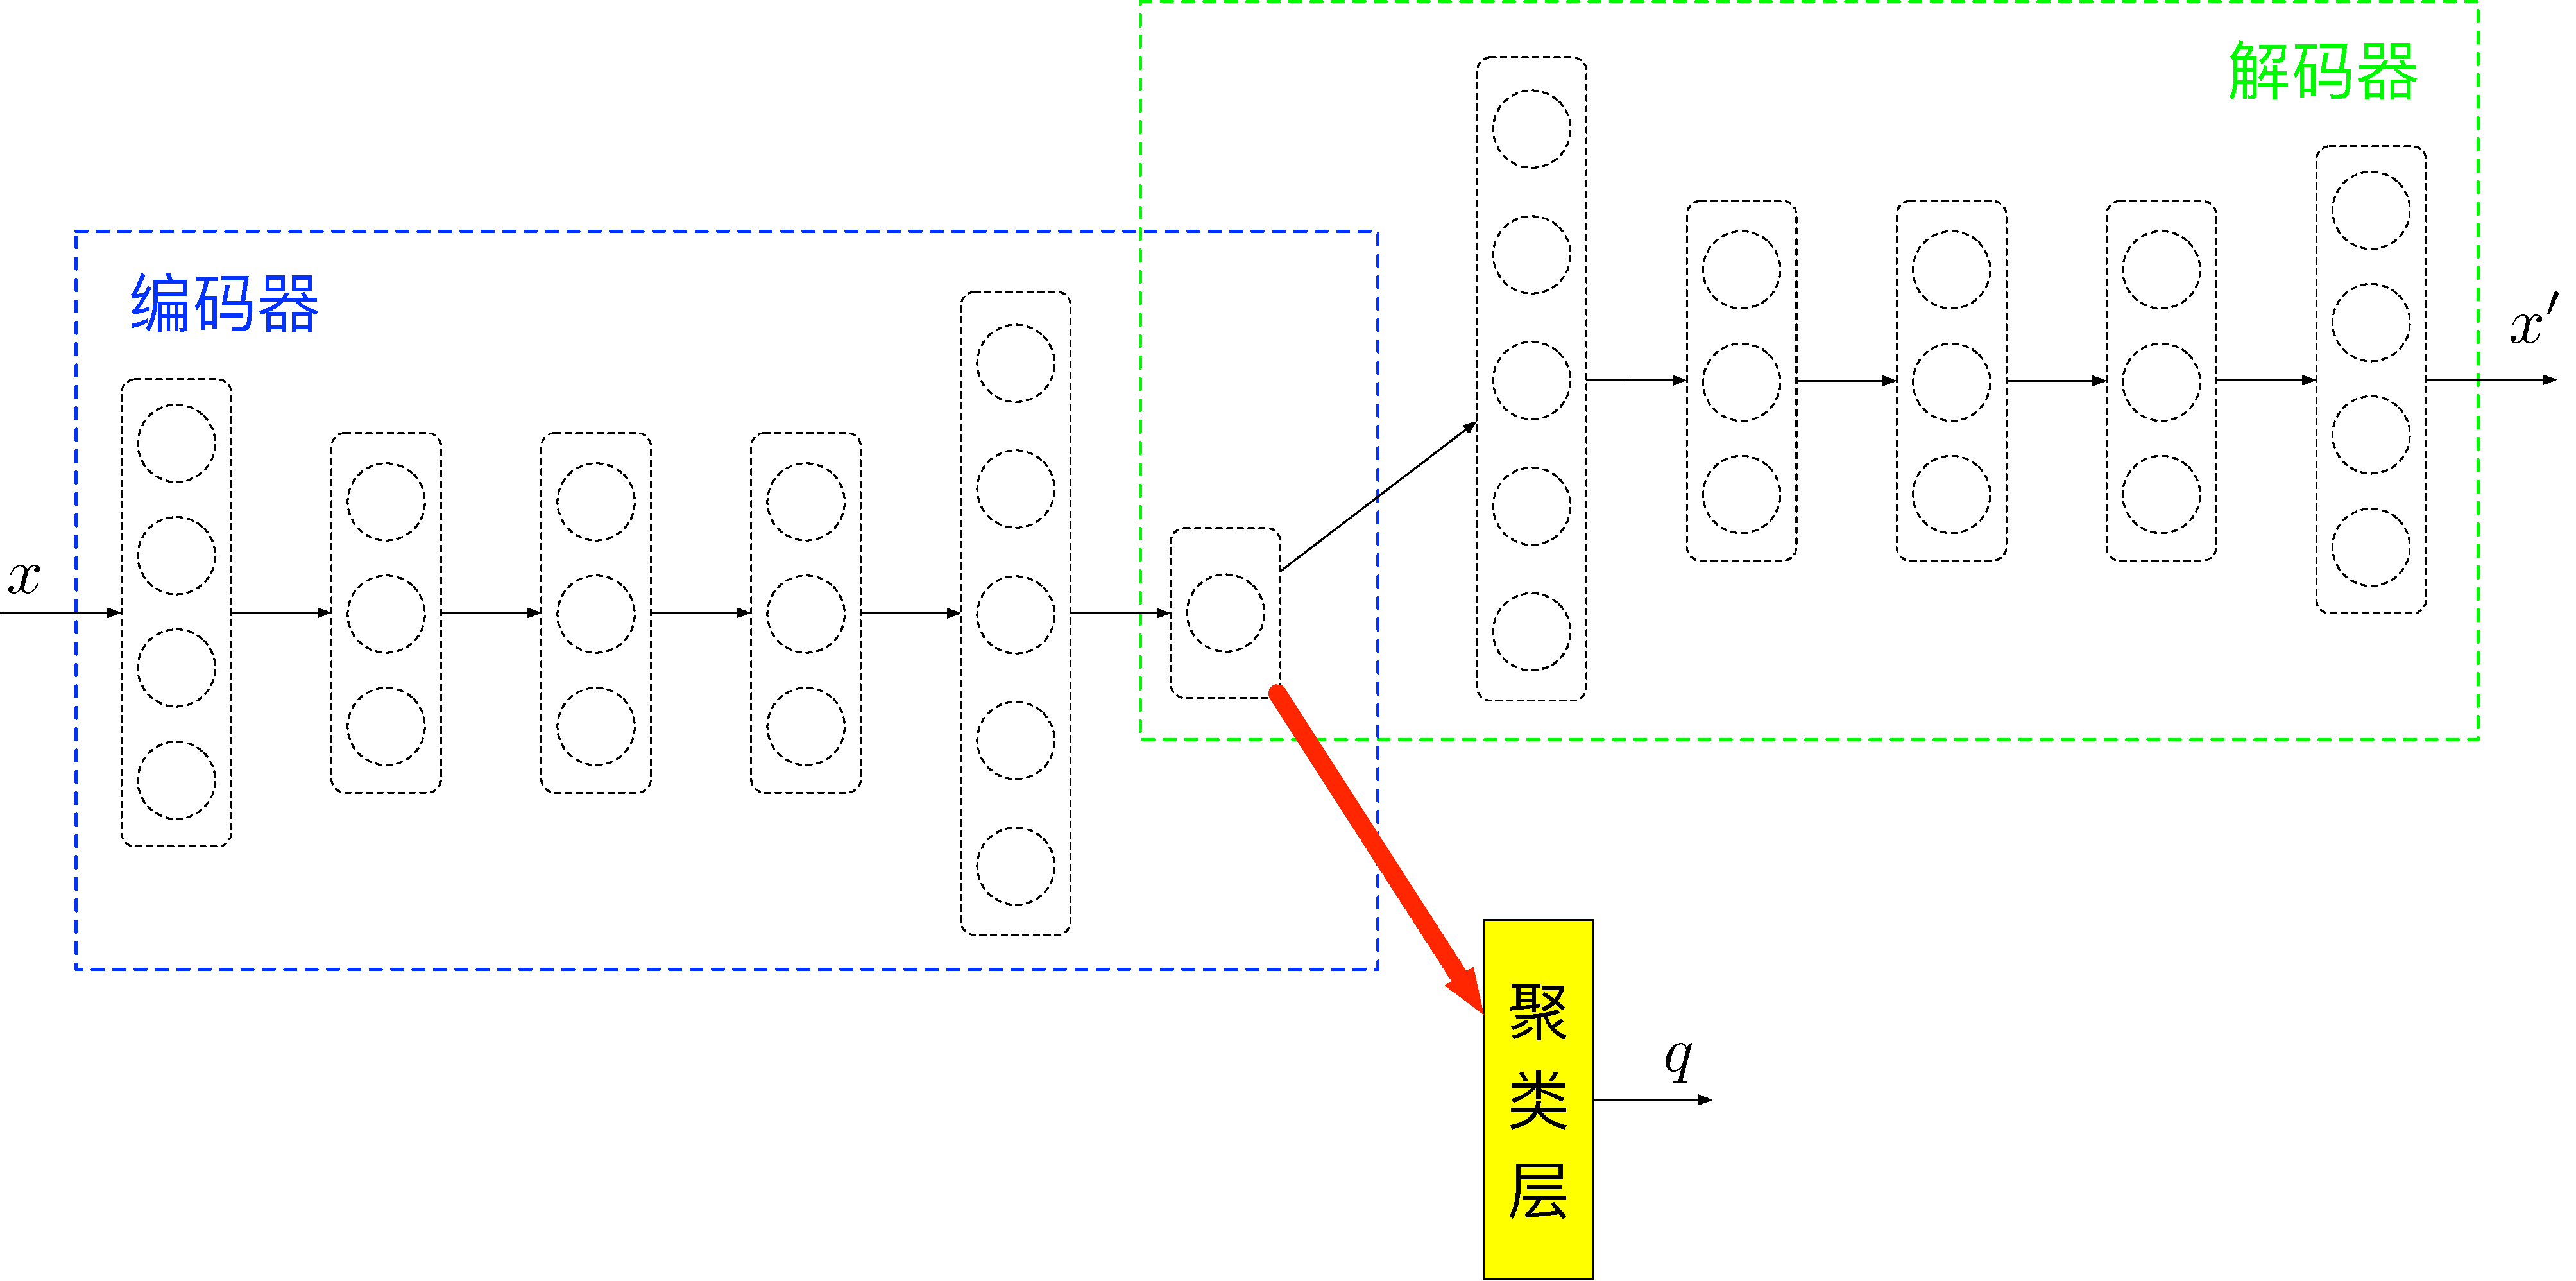
\includegraphics[width=\textwidth]{figures/AE/decc}
	\caption{深度嵌入卷积自编码器结构图}
	\label{fig:decc}
\end{figure}

\subsection{KL散度聚类方法}

文献\cite{maaten2008visualizing}利用学生t分布来衡量嵌入点$z_i$与聚类中心点$\mu_k$的相似度:
\begin{equation}
	p_{ik}=\frac{(1+||z_i-\mu_k||^2/\alpha)^{-\frac{\alpha+1}{2}}}{\sum_{k'}(1+||z_i-\mu_k||^2/\alpha)^{-\frac{\alpha+1}{2}}}
\end{equation}
其中,$\alpha$为学生t分布的自由度,$p_{ik}$可以看作样本$i$到类别$k$的概率。

为了定义我们的聚类目标函数,我们使用辅助目标变量(auxiliary target variable)$Q$来迭代地改进模型预测。为此,我们首先使用Kullback-Leibler(KL)散度来减小模型预测$P$和目标分布$Q$之间的距离。
\begin{equation}
\mathscr{L}_{kld}=KL(Q||P)=\frac{1}{N}\sum_{i=1}^{N}\sum_{k=1}^{K}q_{ik}\log{\frac{q_{ik}}{p_{ik}}}
\label{equ:kldfirst}
\end{equation}
根据文献\cite{xie2016unsupervised},目标分布$Q$的定义如下:
\begin{equation}
	q_{ij}=\frac{p_{ij}^2/f_k}{\sum_k(p_{ik}^2/f_k)}
\end{equation}
其中$f_k$的定义为
\begin{equation}
	f_k=\sum_iq_{ik}
\end{equation}

公式\ref{equ:mse}给出了自编码器重构的损失函数,故最终的损失函数为:
\begin{equation}
	\mathscr{L}=\mathscr{L}_{mse}+\beta \mathscr{L}_{kld}
\end{equation}
其中,$\beta > 0$为调节两部分损失函数的权重。

\section{仿真验证}
\subsection{参数设置}
本章根据如图设计的卷积自编码器进行特征的降维,该部分进行30次迭代,学习方法为Adam。然后利用随机20次k均值算法然后从中选取最优结果,作为起始的聚类中心点,此也作为我们的一个对比算法。损失函数的权重系数$\beta = 0.1$,学生t的自由度$\alpha = 1$。
% 在后续的
最终的优化问题可以通过小批量随机梯度下降和反向传播得到有效解决。

\subsection{仿真结果分析}
我们利用第三章中组C的训练数据用于本章的实验。其实验结果如表\ref{tab:uns}所示。
\begin{table}[H]
	\renewcommand{\arraystretch}{1.3}
	\caption{辐射源信号数据}
	\label{tab:uns}
	\centering
	\begin{tabularx}{\textwidth}{>{\centering\arraybackslash}X>{\centering\arraybackslash}X>{\centering\arraybackslash}X}
		\hline
		 方法 & 无监督聚类精度 & 时间  \\
		 \hline
		CAE + k均值 & $66\%$ & 12\\
		DECC($\beta=0$) & $23\%$ & 12 \\
		DECC & $453\%$ & 12\\
		 \hline
	\end{tabularx}
\end{table}
此处无监督聚类精度(unsupervised clustering accuracy, ACC)的定义为:
\begin{align}
	ACC &= \max\limits_m\frac{\sum_{i=1}^ng(l_i,m(c_i))}{n} \\
	g(l_i,m(c_i)) &= \left\{
		\begin{array}{rcl}
		1       &      & l_i = m(c_i)\\
		0       &      & l_i \neq m(c_i)
		\end{array} \right. \nonumber
\end{align}
其中,$l_i$为真实的标签,$c_i$为算法的聚类结果,$m$是聚类结果与实际标签类别之间的一一对应,其遍历所有可能假设。
\section{小结}
本章结合卷积神经网络与自编码器提出了深度嵌入卷积聚类方法DECC。其通过在损失函数中将KL散度与重构损失两部分结合,使得本章的算法对于两部分可能都进行了考虑。

虽然与有监督学习算法相比,本章的算法精度仍然不够高,但是相比于传统的聚类算法精度有了一定的提高。在一定程度上可以减少打标签的过程。

本章的贡献是:
\begin{itemize}
	\item 可以以端对端方式训练的卷积自编码器被设计用于从未标记的数据中学习特征。通过在杂波数据中包含空间、时间信息,设计了好于传统堆栈自编码器的卷积自编码器。实验结果证明卷积层、卷积转置层和完全连通层足以构建一个有效的CAE。
	\item 在根据聚类损失函数调整网络参数时考虑局部结构特征。实验结果证明,利用局部结构特征有助于稳定训练过程。
	\item 我们提出了深度嵌入卷积聚类算法来自动聚类地海杂波。DECC利用CAE提取局部特征的优势。
	\item 利用天波超视距雷达的实际地海杂波数据进行了实验,结果验证了DECC算法的有效性。
\end{itemize}



% 为了避免退化解,即将大部分样本分配给几个类别或者将某个类别分配给异常样本,我们给目标变量添加一个正则化项。为此,我们参考文献\cite{dizaji2017deep}定义目标变量的分布为:

% 其中$f_k$可以被认为是目标分布中聚类分配的软频率。
% 根据此分布,我们可以将公式\ref{equ:kldfirst}中的损失函数变为下式:
% \begin{align}
% 	\mathscr{L_{kld}}&=KL(Q||P)+KL(f||u) \\
% 	&=[\frac{1}{N}\sum_{i=1}^{N}\sum_{k=1}^{K}q_{ik}\log{\frac{q_{ik}}{p_{ik}}}]+[\frac{1}{N}\sum_{k=1}^{K}f_k\log{\frac{f_k}{u_k}}] \nonumber\\
% 	&=\frac{1}{N}\sum_{i=1}^{N}\sum_{k=1}^{K}q_{ik}\log{\frac{q_{ik}}{p_{ik}}}+q_{ik}\log{\frac{f_k}{u_k}} \nonumber
% \end{align}
% 其中$u$是经验标签分布的先验分布。损失函数的第一项使目标和模型预测分布之间的距离最小,第二项平衡了目标变量中的类别的频率。
% 因此,我们可以间接地使得最终模型可以具有更平衡的聚类。一般情况下,$u$可以设为均匀分布,当然也可以根据先验知识对其进行调整。

% 此处利用联合优化的思想对参数进行求解。首先通过固定参数来估计目标变量$Q$,然后再利用该目标变量更新参数。则可以得到下述优化问题:
% \begin{equation}
% \min \limits_{Q}\frac{1}{N}\sum_{i=1}^{N}\sum_{k=1}^{K}q_{ik}\log{\frac{q_{ik}}{p_{ik}}}+q_{ik}\log{\frac{f_k}{u_k}}
% \end{equation}

% %where the target variables are constrained to  k qik = 1. This problem can be solved using first order methods, such as gradient descent, projected gradient descent, and Nes- terov optimal method [24], which only require the objective function value and its (sub)gradient at each iteration. In the following equation, we show the partial derivative of the objective function with respect to the target variables.
% 其中,目标变量被约束为$\sum_k{q_{ik}}=1$。
% 这个问题可以用一阶方法求解,如梯度下降法,投影梯度下降法和奈斯托夫最优化方法[24],只需要目标函数值 (子)梯度在每次迭代。在下面的等式中,我们显示了目标函数相对于目标变量的偏导数。
% \begin{equation}
% \frac{\partial\mathscr{L}}{\partial{q_{ik}}}\propto\log(\frac{q_{ik}f_k}{p_{ik}})+\frac{q_{ik}}{\sum_{i'=1}^{N}q_{i'k}}+1
% \end{equation}
% Investigating this problem more carefully, we approximate the gradient in Eq.(6) by removing the second term, since the number of samples N is often big enough to ignore the second term. Setting the gradient equal to zero, we are now able to compute the closed form solution for Q accordingly.
% \begin{equation}
% q_{ik}=\frac{p_{ik}/(\sum_{i'}p_{i'k})^{\frac{1}{2}}}{\sum_{k'}p_{ik'}/(\sum_{i'}p_{i'k'})^{\frac{1}{2}}}
% \end{equation}
% For the maximization step, we update the network parameters $\psi=\{\Theta, W\}$ using the estimated target variables with the following objective function.
% \begin{equation}
% \min\limits_{\psi} \space -\frac{1}{N}\sum_{i=1}^{N}\sum_{k=1}^{K}q_{ik}\log{p_{ik}}
% \end{equation}

% %Interestingly, this problem can be considered as a standard cross entropy loss function for classification tasks, and the parameters of soft-max layer Θ and embedding function W can be efficiently updated by backpropagating the error.
% %
% %As a crucial point, DEPICT algorithm provides a joint learning framework that optimizes the soft-max and autoencoder parameters together.
% %
% 有趣的是,这个问题可以看作是分类任务的标准交叉熵损失函数,软-max层参数和嵌入函数W可以通过反向传播错误来有效地更新。